\documentclass[a4paper,12pt]{article} % добавить leqno в [] для нумерации слева

% Для кода
\usepackage{listings}
\usepackage{color}

\definecolor{dkgreen}{rgb}{0,0.6,0}
\definecolor{gray}{rgb}{0.5,0.5,0.5}
\definecolor{mauve}{rgb}{0.58,0,0.82}

\lstset{frame=tb,
  language=Java,
  aboveskip=3mm,
  belowskip=3mm,
  showstringspaces=false,
  columns=flexible,
  basicstyle={\small\ttfamily},
  numbers=none,
  numberstyle=\tiny\color{gray},
  keywordstyle=\color{blue},
  commentstyle=\color{dkgreen},
  stringstyle=\color{mauve},
  breaklines=true,
  breakatwhitespace=true,
  tabsize=3
}

%%% Работа с русским языком
\usepackage{cmap}					% поиск в PDF
\usepackage{mathtext} 				% русские буквы в формулах
\usepackage[T2A]{fontenc}			% кодировка
\usepackage[utf8]{inputenc}			% кодировка исходного текста
%\usepackage[english,russian]{babel}	% локализация и переносы
\usepackage[english]{babel}

\usepackage{pdfpages}

%%% Дополнительная работа с математикой
\usepackage{amsmath,amsfonts,amssymb,amsthm,mathtools} % AMS

\usepackage{icomma} % "Умная" запятая: $0,2$ --- число, $0, 2$ --- перечисление

%% Номера формул
%\mathtoolsset{showonlyrefs=true} % Показывать номера только у тех формул, на которые есть \eqref{} в тексте.

%% Шрифты
\usepackage{euscript}	 % Шрифт Евклид
\usepackage{mathrsfs} % Красивый матшрифт

%% Свои команды
%\DeclareMathOperator{\sgn}{\mathop{sgn}}

%% Перенос знаков в формулах (по Львовскому)
%\newcommand*{\hm}[1]{#1\nobreak\discretionary{}
%{\hbox{$\mathsurround=0pt #1$}}{}}

%%% Работа с картинками
\usepackage{graphicx}  % Для вставки рисунков
\graphicspath{{images/}{images2/}}  % папки с картинками
\setlength\fboxsep{3pt} % Отступ рамки \fbox{} от рисунка
\setlength\fboxrule{1pt} % Толщина линий рамки \fbox{}
\usepackage{wrapfig} % Обтекание рисунков и таблиц текстом
\usepackage{float} % H - here опция

%%% Работа с таблицами
\usepackage{array,tabularx,tabulary,booktabs} % Дополнительная работа с таблицами
\usepackage{longtable}  % Длинные таблицы
\usepackage{multirow} % Слияние строк в таблице

%%% Заголовок
\author{Sergei Vostrikov}
\title{Eurobot 2019 manual for EE team}
\date{\today}

\begin{document} % конец преамбулы, начало документа

\maketitle

\newpage
\section*{Introduction}
Eurobot is an international robotics competition for students. The team REset of Skoltech regularly participates in the contest since 2014. Each year on a basis of competition ISP lab selects new team members from the $1^{st}$ year MSc students to form new team. In such conditions the key component of team's development is an effective transfer of knowledge between the generations. This document is a short guide for a STM 32 firmware that was developed by the Eurobot 2018 team. The paper is organised in a following way. In a first section the author makes an overview of used architecture to presenting breakdown structure of the firmware. In the following sections subsytems are described in a more detailed way.

\section{Breakdown structure of the firmware}
The breakdown structure of the firmware for STM32f4 microcontroller is represented in the figure \ref{ris:scheme}. 

The pattern of a superloop with interrupts is used to implement all necessary functionality. After power on all the peripheral modules are initialized at beginning of \textit(int main()). Then inside a "while" loop (main.c) we can observe only functions that are responsible for two tasks:
\begin{itemize}
	\item Communication with high level.
	\item Global shutdown.
\end{itemize}
All other tasks are implemented inside interrupt handlers of timer modules. They are:
\begin{itemize}
	\item Movement control.
	\item Collision avoidance control.
	\item Task execution of servo manipulators.
	\item Global timer update.
\end{itemize}
In the next subsections each subsystem will be shortly described and mapped to concrete files where the functionality is implemented.

\begin{figure}[H]
\center{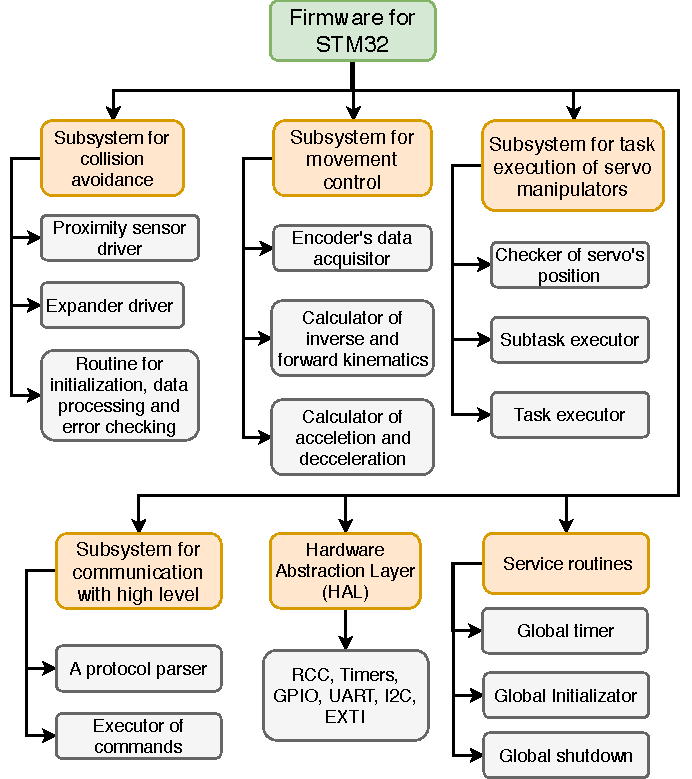
\includegraphics[scale = 1.0]
{scheme}}
\caption{The breakdown structure.}
\label{ris:scheme}
\end{figure}

\subsection{Subsystem for collision avoidance}
The collision avoidance system of the robot is based on a set of proximity sensors \textit{VL6180X} from \textit{ST} company. It is a time of flight (TOF) sensor that has an approximate precision (noise) of $2\:mm$ and typical accuracy (range offset for surfaces with different reflectance) of about $13\:mm$. The sensor has digital I2C interface with a fixed I2C adress that can be changed after power on. As we are using a set of sensor with the same initial adress the subsystem also contains GPIO I2C expander \textit{MCP23017}. The expander allows to perform subsequent initialization of sensor's array and local reinitialization of particular sensor in case of an error. The maximum frequency of sensor's data acquisition for one sensor depends on the reflectance of the target, but it could be configured with constrained convergence time (see the datasheet for \textit{VL6180X}). In the firmware a custom method of sensor's initialization is used that allows to achieve $50 Hz$ data acquisition frequency and reduce the sensitivity cone for the proximity sensors. 

The source code files for  \textit{VL6180X} driver:
\begin{itemize}
	\item \textbf{\textit{VL6180x.h}}
	\item \textbf{\textit{VL6180x.c}}
\end{itemize}

The source code files for  \textit{MCP23017} driver and other subroutines:
\begin{itemize}
	\item \textbf{\textit{Collision\_avoidance.h}}
	\item \textbf{\textit{Collision\_avoidance.c}}
\end{itemize}

Periodical data acquisition of ranges is implemented in the interrupt handler of a timer called \textbf{\textit{COLL\_AVOID\_TIM\_MODULE}}. The code of the handler is located in \textbf{\textit{Interrupts.c}}.

\subsection{Subsystem for movement control}

\subsection{Subsystem for task execution of servo manipulators}

\subsection{Subsystem for communication with high level}

\subsection{Service Routines}

\subsection{Hardware abstraction layer (HAL)}

%\section*{\hfil Instructions \hfil}

%    \begin{lstlisting}
%	typedef union {
%		uint64_t raw;
%		struct {
%				uint8_t prescaler;
%				uint32_t clock;
%				uint16_t comp;
%				};
%	} timer_desc;
%	\end{lstlisting}

\end{document} % конец документа

